\chapter{Numerical Characterization of Acoustic Radiation Force Impulse Imaging}
	\label{chap:arfi}
	\section{Introduction}
		Acoustic radiation force impulse imaging presents a chief benefit over quasi-static ultrasound elastography in that since the external deformation force is applied by the transducer itself rather than through manual indentation of the transducer by the diagnostician, the inter-operator reliability may be greatly increased. The net effect of this is an expected decrease in the required amount of training of diagnosticians as well as an expected increase in the sensitivity and specificity of early deep tissue injury detection.

	\section{Method}
	\label{sec:arfi_methods}
		In order to numerically characterize acoustic radiation force impulse imaging for the early detection of deep tissue injuries, a combinatory model of acoustic radiation force simulations and time-domain finite-element models of tissue deformation were used. Acoustic radiation force distributions were calculated using a k-space pseudo-spectral model of ultrasonic acoustics which simulated the acoustic intensities and subsequent radiation force developed by an ultrasonic transducer applying deep body loads to soft tissue. These forces were then combined with a temporal finite-element model of tissue deformation to model the response of the tissue to the body force impulses generated by the transducer. The use of these models allowed extensive simulation and parameter sensitivity analysis in order to numerically characterize the use of acoustic radiation force impulse imaging for detecting deep tissue injuries.

		\subsection{K-Space Pseudo-spectral Model of Acoustic Fields}
		\label{subsec:kspace_model}
			In order to simulate the body loads generated within deep tissue by a continuous ultrasound beam, a k-space pseudo-spectral model of acoustic field intensities was generated. The body load fields that were generated as a result of this model were fed into a temporal soft tissue deformation model to investigate the dynamic response of tissue to ARFI loads.

			The governing equations used for the k-space pseudo-spectral model were the set of coupled first-order partial differential equations \ref{equ:arfi_gov_p1} -- \ref{equ:arfi_gov_p3}. These equations are the first-order equivalents of the wave equation given in equation \ref{equ:wave_equation} taking into account acoustic absorption, tissue heterogeneities, and acoustic wave non-linearities \cite{treeby12}. Equations \ref{equ:arfi_gov_p1}, \ref{equ:arfi_gov_p2}, and \ref{equ:arfi_gov_p3} represent the momentum conservation, mass conservation, and pressure-density relation terms respectively.

			\begin{subequations}
				\label{equ:arfi_gov}
				\begin{align}
					\frac{\partial \vec{v}}{\partial t} &= - \frac{1}{\rho_0} \nabla p \label{equ:arfi_gov_p1} \\
					\frac{\partial p}{\partial t} &= -\left(2 \rho + \rho_0\right)\nabla \cdot \vec{v} - \vec{v} \cdot \nabla \rho_0 \label{equ:arfi_gov_p2} \\
					p &= c_0^2 \left(\rho + \vec{u} \cdot \nabla \rho_0 + \frac{B}{2A} \frac{\rho^2}{\rho_0} - \mathbf{L}\rho \right) \label{equ:arfi_gov_p3}
				\end{align}
			\end{subequations}

			In equations \ref{equ:arfi_gov}, $\vec{v}$ is the acoustic particle velocity, $p$ is the acoustic pressure, $\rho$ is the acoustic density, $\rho_0$ is the equilibrium density, $c_0$ is the acoustic sound speed, $\vec{u}$ is the acoustic particle displacement, and $\sfrac{B}{A}$ is a nonlinearity parameter which models alterations to the sound speed \cite{beyer08}.

			\begin{equation}
				\label{equ:wave_equation}
				\nabla^2 p - \frac{1}{c_0^2}\frac{\partial^2 p}{\partial t^2} = 0
			\end{equation}

			The $\mathbf{L}$ operator used in equation \ref{equ:arfi_gov_p3} accounts for acoustic absorption and dispersion which follows a frequency power law and is defined as per equations \ref{equ:Lop1} -- \ref{equ:Lop3} where $\alpha_0$ is the power law prefactor and $y$ is the power law exponent of the tissue. $\tau$ and $\eta$ represent absorption and dispersion proportionality coefficients respectively.

			\begin{subequations}
				\begin{align}
					\mathbf{L} &= \tau \frac{\partial}{\partial t}\left(-\nabla^2\right)^{\frac{y}{2} - 1} + \eta \left(-\nabla^2\right)^{\frac{y+1}{2} - 1} \label{equ:Lop1} \\
					\tau &= -2\alpha_0 c_0^{y-1} \label{equ:Lop2} \\
					\eta &= 2\alpha_0c_0^y\tan\left(\frac{\pi y}{2}\right)  \label{equ:Lop3}
				\end{align}
			\end{subequations}

			In order to integrate pressure sources in equations \ref{equ:arfi_gov_p1} -- \ref{equ:arfi_gov_p3}, equation \ref{equ:arfi_gov_p2} is modified to include a mass source term, $S_M$ which counts as a pressure source term through changing density to form equation \ref{equ:arfi_gov_p2_source}.

			\begin{equation}
				\label{equ:arfi_gov_p2_source}
				\frac{\partial p}{\partial t} = -\left(2 \rho + \rho_0\right)\nabla \cdot \vec{v} - \vec{v} \cdot \nabla \rho_0 + S_M
			\end{equation}

			The k-Wave MATLAB\textsuperscript{\textregistered} toolbox version 1.0 was used to solve for the time-variant intensities resulting from simulated acoustic radiation force impulses applied to heterogeneous soft tissue using equations \ref{equ:arfi_gov_p1}, \ref{equ:arfi_gov_p2_source}, and \ref{equ:arfi_gov_p3} with the acoustic properties listed in Table \ref{tab:kspace_properties}. Sample source code for performing these simulations using the k-Wave toolbox is given in listing \ref{lst:intensity} in Appendix \ref{app:source_code}.

			\begin{table}[!htb]
				\centering
				\caption{K-Space pseudo-spectral model parameters}
				\label{tab:kspace_properties}
				\begin{tabular}{llSs[table-unit-alignment = left]}
					\toprule
					Property & Symbol & {Value} & Units \\
					\midrule
					Nonlinearity parameter & $\sfrac{B}{A}$ & 8 & - \\
					Power law prefactor & $\alpha_0$ & 0.7 & $\si{\neper} \left(\si{rad\per\s}\right)^{-y} \si{\per\m}$ \\
					Power law exponent & $y$ & 0.95 & - \\
					Density & $\rho_0$ & 1060 & \si{\kg\per\m\cubed} \\
					\bottomrule
				\end{tabular}
			\end{table}

		\subsection{Derivation of Acoustic Radiation Force}
		\label{subsec:body_load_derivation}
			Acoustic radiation force arises as the result of absorption of linear momentum within tissue as acoustic waves travel though it with the requirement that the tissue is a viscoelastic medium---no energy would be absorbed in a purely linear elastic model. Further, at the super-\si{\MHz} frequencies involved in ultrasound interrogation, tissue may be considered a viscous fluid \cite{palmeri05}.

			Using a perturbative expansion of the general equation of linear momentum given in equation \ref{equ:arfi_linear_momentum}, acoustic radiation force can be expressed as per equations \ref{equ:radiation_force_1} \cite{nyborg65}. In equations \ref{equ:radiation_force_1}, $\langle\rangle$ represents the time-average operator, $\vec{v_1}$ and $\vec{v_2}$ are the first and second order terms in the perturbative expansion of particle velocity, $p_2$ is the second order pressure term in the perturbative expansion, while $\vec{F}$ represents the acoustic radiation force developed in the tissue.

			\begin{equation}
				\label{equ:arfi_linear_momentum}
				\sigma_{ij,j} + \rho b_i = \rho f_i
			\end{equation}

			\begin{subequations}
				\label{equ:radiation_force_1}
				\begin{align}
					\vec{F} &= \nabla p_2 - \mu_{tissue} \nabla^2 \vec{v_2} \label{equ:radiation_force_1a} \\
					\vec{F} &= \rho \langle\vec{v_1}\nabla\cdot\vec{v_1} + \vec{v_1}\nabla\vec{v_1}\rangle \label{equ:radiation_force_1b}
				\end{align}
			\end{subequations}

			For a plane wave, equation \ref{equ:radiation_force_1b} can be reduced to equation \ref{equ:radiation_force_2}. Further, substituting the generalized wave particle velocity solution given in equation \ref{equ:particle_velocity} in equation \ref{equ:radiation_force_2}, the magnitude of acoustic radiation force may be calculated as per equation \ref{equ:radiation_force_3}.

			\begin{equation}
				\label{equ:radiation_force_2}
				\vec{F} = 2\rho\langle \vec{v} \vec{v}_{,x} \rangle
			\end{equation}

			\begin{equation}
				\label{equ:particle_velocity}
				\vec{v} = i\omega A e^{-\alpha x + i\left(\omega t - k x\right)}\hat{x}
			\end{equation}

			\begin{equation}
				\label{equ:radiation_force_3}
				\left|\vec{F}\right| = A^2 e^{-2\alpha x}\rho\alpha
			\end{equation}

			Further using the acoustic field intensity, the acoustic radiation force may be calculated as per equation \ref{equ:radiation_force} where $\alpha$ is the absorption coefficient of the tissue in \si{\neper\per\m}, $I$ is the temporal average acoustic intensity in \si{\W\per\m\squared}, and $c$ is the longitudinal speed of sound in the tissue in \si{\m\per\s} \cite{palmeri05}.

			\begin{equation}
				\label{equ:radiation_force}
				\left|\vec{F}\right| = \frac{2\alpha I}{c}
			\end{equation}

			Once acoustic radiation force body loads were calculated as per equation \ref{equ:radiation_force}, they were used as initial conditions to the temporal finite-element model of soft tissue deformation described in Section \ref{subsec:temporal_fea_arfi}.

		\subsection{Temporal Finite-Element Model of Soft Tissue Deformation}
			\label{subsec:temporal_fea_arfi}
			In response to the relatively short duration (``impulse'') acoustic radiation force body load applied to tissue in ARFI imaging, the interrogated tissue will exhibit a dynamic response---namely that tissue deformation will propagate outwards as the absorbed acoustic energy diffuses through the soft tissue.

			In order to simulate the dynamic tissue deformation generated by the acoustic impulse force, a generalized Maxwell viscoelastic model of tissue deformation was used \cite{then12}. The simulated tissue properties are summarized in Tables \ref{tab:arfi_properties} and \ref{tab:arfi_maxwell_properties}.

			\begin{table}[!htb]
				\centering
				\caption{ARFI model tissue properties}
				\label{tab:arfi_properties}
				\begin{tabular}{llSs[table-unit-alignment = left]}
					\toprule
					Property & Symbol & {Value} & Units \\
					\midrule
					Bulk Modulus & $K$ & 515.7 & \si{\kPa} \\
					Shear Modulus & $\mu_{tissue}$ & 1.0 & \si{\kPa} \\
					Density & $\rho$ & 1060 & \si{\kg\per\m\cubed} \\
					\bottomrule
				\end{tabular}
			\end{table}

			\begin{table}[!htb]
				\centering
				\caption{ARFI Maxwell model tissue properties}
				\label{tab:arfi_maxwell_properties}
				\begin{tabular}{SSS}
					\toprule
					{Branch} & {Shear Modulus} & {Relaxation Time} \\
					& {(\si{\Pa})} & {(\si{\s})} \\
					\midrule
					1 & 791.0 & 2 \\
					2 & 66.5 & 40 \\
					3 & 0.6 & 80 \\
					\bottomrule
				\end{tabular}
			\end{table}

			The time-dependent displacement fields were calculated according to equation \ref{fea:time_deformation} where $\sigma$ is the Cauchy stress tensor, $\vec{F}$ are the applied body forces, and $\vec{u}$ is the particle displacement, and $\rho$ is the density.

			\begin{equation}
				\label{fea:time_deformation}
				\rho \frac{\partial^2 \vec{u}}{\partial t^2} - \nabla \cdot \sigma = \vec{F}
			\end{equation}

			In order to include viscoelastic effects through a generalized Maxwell model of soft tissue, equation \ref{fea:time_deformation_visco} was used where $\sigma_0$ is the initial stress distribution in the tissue, $C$ is the $4^{\text{\tiny th}}$ order elasticity tensor, $\varepsilon$ is the strain, $G_m$ and $\tau_m$ are the shear modulus and relaxation time of the $m^{\text{\tiny th}}$ branch of the Maxwell model respectively, and $\gamma_m$ is an additional auxiliary degree of freedom used to represent the extension of the abstract springs in the Maxwell model.

			\begin{equation}
				\label{fea:time_deformation_visco}
				\sigma - \sigma_0 = C : \varepsilon + \sum_m 2 G_m \tau_m \dot{\gamma}_m 
			\end{equation}

			In the simulations, the boundary equations \ref{equ:arfi_fea_fixed_bc} were used to apply a fixed boundary condition to the both the bottom (deep) and top (superficial) boundaries of the model in the axial direction at both boundaries and in the lateral direction at the deep boundary. All other boundaries of the model were free to translate in all dimensions. A visual representation of these boundary conditions is given in Fig. \ref{fig:arfi:boundary_conditions}. The acoustic radiation force was applied as a body load to the tissue in the model with the distribution calculated by the k-space pseudo-spectral model and resultant body forces described in Sections \ref{subsec:kspace_model} and \ref{subsec:body_load_derivation}. In order to prevent reflections from the model boundaries that might affect the simulation results, the model geometry extended laterally by \SI{5}{\cm} in either direction from the centreline. Simulations were run until the axial displacement at the focal point returned to \SI{1}{\percent} of it's maximal value during the entire simulation---at this point, the tissue was considered to be ``relaxed'' after being disturbed by the acoustic radiation force. Sample source code for calculating these finite-element models using COMSOL Multiphysics\textsuperscript{\textregistered}\  is given in listing \ref{lst:relaxation} in Appendix \ref{app:source_code}.

			\begin{subequations}
				\label{equ:arfi_fea_fixed_bc}
				\begin{align}
					\vec{u} &= 0, \qquad \Gamma = \Gamma_{bottom} \\
					u_y &= 0, \qquad \Gamma = \Gamma_{top}
				\end{align}
			\end{subequations}

			\begin{figure}[!htb]
				\centering
					\begin{tikzpicture}[x=0.045\textwidth, y=0.045\textwidth, draw=black, text=black, fill=black]
						% the main domain area
						\draw[fill=tissueColour] (0, 0) rectangle(10, 10);

						% bottom hold
						\foreach \x in {0.0,0.4,...,9.6}
						{
							\draw (\x, -0.2) -- (\x + 0.2, 0);
						}
						\draw (5, -0.2) node[below] {$\vec{u} = 0$};

						% top rollers
						\foreach \x in {0.2,0.6,...,10}
						{
							\draw(\x, 10.2) circle(0.2);
						}
						\draw (0, 10.4) -- (10, 10.4);
						\draw (5, 10.4) node[above] {$u_y = 0$};

						% body load force arrows
						\draw[->] (6, 7) arc[radius=3, start angle=135, end angle=180];
						\draw[->] (4, 7) arc[radius=3, start angle=45, end angle=0];
						\draw[->] (5.1, 4.75) arc[radius=3, start angle=180, end angle=200];
						\draw[->] (4.9, 4.75) arc[radius=3, start angle=0, end angle=-20];
						\draw (5.1, 5) node[right]{$\vec{F}$};

						% bottom / top boundary labels
						\draw (5, 10) node[below]{$\Gamma = \Gamma_{top}$};
						\draw (5, 0) node[above]{$\Gamma = \Gamma_{bottom}$};

					\end{tikzpicture}
				\caption[ARFI finite-element model boundary conditions]{Boundary conditions used in the finite-element calculations of soft tissue deformation.}
				\label{fig:arfi:boundary_conditions}
			\end{figure}

		\FloatBarrier
		\subsection{Characterizing Acoustic Radiation Force Impulse Imaging}
		\label{subsec:arfi_method_characterization}
			In order to fully understand the suitability of using ARFI imaging to detect and monitor deep tissue injuries, 1 model of unlesioned tissue and 4 general models of deep tissue injury lesions were modelled. Each model was investigated over a range of parameters in order to determine the relationship between the detection sensitivity and the various parameters that were studied. The unlesioned model was used to investigate the general effects of acoustic radiation force impulse forces in soft tissue. The investigated lesionous models included a hard-boundaried spherical lesion embedded in a homogeneous soft tissue domain, a lesion with blurred boundaries that ``fades'' into the homogeneous soft tissue background, a cluster of small lesions which together comprise a greater lesionous region, and a lesion with MRI-acquired geometry \cite{solis13} embedded in geometry obtained from a Visible Human slice \cite{visiblehuman}. Schematics of the four investigated models are given in \ref{fig:arfi_schematics}.

			\begin{figure*}[!htb]
				\centering
				\subfloat[]{
					\begin{tikzpicture}[x=0.045\textwidth, y=0.045\textwidth, draw=black, text=black, fill=black]
						% the main domain area
						\draw[fill=tissueColour] (0, 0) rectangle(10, 10);

						% the lesion
						\draw[fill=lesionColour] (5, 6) circle(0.5);

						% the lesion center marks
						\draw (4.4, 6) -- (4.9, 6);
						\draw (5.1, 6) -- (5.6, 6);
						\draw (4.95, 6) -- (5.05, 6);
						\draw (5, 5.4) -- (5, 5.9);
						\draw (5, 6.1) -- (5, 6.6);
						\draw (5, 5.95) -- (5, 6.05);

						% the lesion radius
						\draw[<-] (5.3536, 5.6464) -- (6, 5);
						\draw (5.85, 5) node[right]{\scriptsize $\diameter S$};

						% the lesion depth
						\draw (4, 6) -- (4.5, 6);
						\draw[<-] (4.25, 10) -- (4.25, 8.25);
						\draw (4.25, 8) node{\scriptsize $d$};
						\draw[->] (4.25, 7.75) -- (4.25, 6);

						% the domain width
						\draw (0, 10.1) -- (0, 10.5);
						\draw[<-] (0, 10.25) -- (4.25, 10.25);
						\draw (5, 10.25) node{\scriptsize \SI{10}{\cm}};
						\draw[->] (5.75, 10.25) -- (10, 10.25);
						\draw (10, 10.1) -- (10, 10.5);

						% the domain depth
						\draw (10.1, 0) -- (11, 0);
						\draw[<-] (10.75, 0) -- (10.75, 4.75);
						\draw (10.75, 5) node{\scriptsize \SI{10}{\cm}};
						\draw[->] (10.75, 5.25) -- (10.75, 10);
						\draw (10.1, 10) -- (11, 10);

					\end{tikzpicture}
					\label{fig:arfi_schematic_single}
				}
				~
				\subfloat[]{
					\begin{tikzpicture}[x=0.045\textwidth, y=0.045\textwidth, draw=black, text=black, fill=black]
						% the main domain area
						\draw[fill=tissueColour] (0, 0) rectangle(10, 10);

						% the lesion
						\draw (5, 6) node{
\includegraphics[width=0.045\textwidth]{assets/arfi/images/blurredLesion.png}};
						\draw (5, 6) circle(0.5);

						% the lesion radius
						\draw[<-] (5.3536, 5.6464) -- (6, 5);
						\draw (5.85, 5) node[right]{\scriptsize $\diameter S$};

					\end{tikzpicture}
					\label{fig:arfi_schematic_blur}
				}
				
				\subfloat[]{
					\begin{tikzpicture}[x=0.045\textwidth, y=0.045\textwidth, draw=black, text=black, fill=black]
						% the main domain area
						\draw[fill=tissueColour] (0, 0) rectangle(10, 10);

						% the lesion
						\draw (5, 6) node{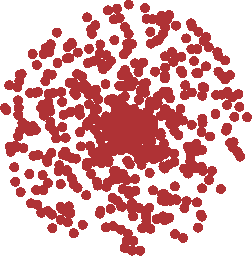
\includegraphics[width=0.045\textwidth]{assets/arfi/images/clusteredLesion.png}};
						\draw (5, 6) circle(0.5);

						% the lesion radius
						\draw[<-] (5.3536, 5.6464) -- (6, 5);
						\draw (5.85, 5) node[right]{\scriptsize $\diameter S$};

						% blob size
						\draw[<-] (4.9, 5.9) -- (4, 5) node[left]{\scriptsize $r_{bl}$};

					\end{tikzpicture}
					\label{fig:arfi_schematic_clustered}
				}
				~
				\subfloat[]{
					\begin{tikzpicture}[x=0.045\textwidth, y=0.045\textwidth, draw=black, text=black, fill=black]
						% the human stuffz
						\draw (5, 5) node{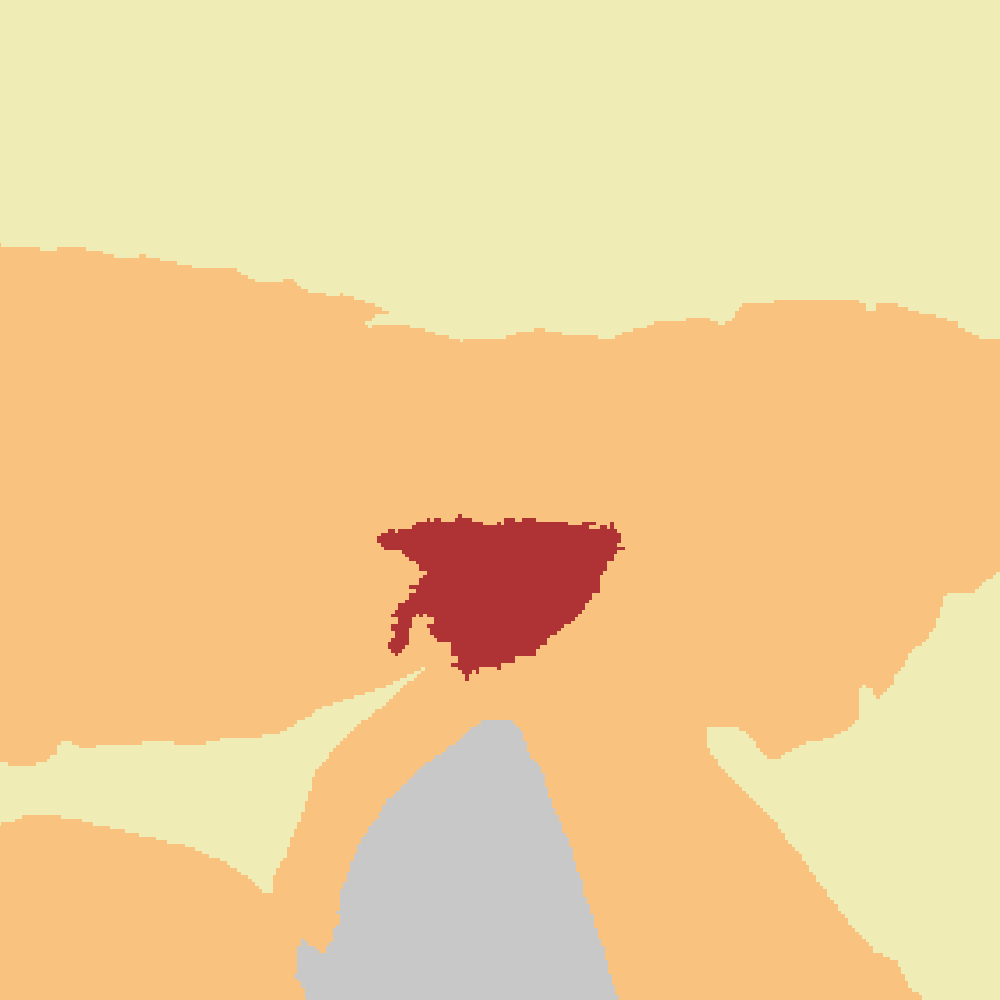
\includegraphics[width=0.45\textwidth]{assets/arfi/images/humanSchematic.png}};

						% the main domain area
						\draw (0, 0) rectangle(10, 10);

						% the depth
						\draw (6, 4) -- (6.75, 4);
						\draw (6.5, 7) node{\scriptsize $d$};
						\draw[<-] (6.5, 10) -- (6.5, 7.25);
						\draw[->] (6.5, 6.75) -- (6.5, 4);

						% the size
						\draw (3.75, 4.7) -- (3.75, 5.5);
						\draw (6.25, 4.7) -- (6.25, 5.5);
						\draw (4.875, 5.25) node{\scriptsize $\diameter L$};
						\draw[<-] (3.75, 5.25) -- (4.5, 5.25);
						\draw[->] (5.25, 5.25) -- (6.25, 5.25);

					\end{tikzpicture}
					\label{fig:arfi_schematic_human}
				}
				\caption[ARFI model schematics]{Schematics of the lesion models that were investigated using acoustic radiation force impulse imaging showing \protect\subref{fig:arfi_schematic_single} a spherical hard-boundaried lesion, \protect\subref{fig:arfi_schematic_blur} a spherical blurred-boundary lesion, \protect\subref{fig:arfi_schematic_clustered} a cluster of numerous small lesions composing a larger lesionous region, and \protect\subref{fig:arfi_schematic_human} the geometry from an MRI-acquired deep tissue injury overlaid on a slice from the Visible Human Project such that the injury lesion was located immediately superior to an ischial tuberosity.}	
				\label{fig:arfi_schematics}
			\end{figure*}

			In order to characterize ARFI imaging, ranges of parameters pertinent to each investigated model were studied. The parameters relating to general soft tissue response to acoustic body loads included: the ARFI interrogation frequency used to excite the tissue with acoustic radiation force; the transducer width which applies the acoustic radiation force to the tissue; the number of pulse cycles (loading time) applied by the transducer; and the pressure applied by the transducer. The lesionous models investigated yet more parameters including: lesion depth; lesion diameter; lesion relative stiffness ratio; lesion blur radius; the number of tightly-packed lesions in a clustered lesion model; the radii of the individual tightly-packed lesions in a clustered lesion model; and the width (and overall size) of the MRI-acquired lesion in the Visible Human model. The range of values of these investigated parameters are listed in Table \ref{tab:arfi-parametervalues}.

			\begin{table}[!htb]
				\centering
				\caption[ARFI model investigated parameters]{Range of values of investigated parameters in the various ARFI models that were studied.}
				\label{tab:arfi-parametervalues}
				\begin{tabular}{lccs[table-unit-alignment = left]}
					\toprule
					Parameter & Symbol & Values & {Units} \\
					\midrule
					ARFI interrogation frequency & $f$ & \numlist{1;2;4;6} & \MHz \\
					Transducer width & $w_{trans}$ & \numlist{4;8;10} & \cm \\
					ARFI pulse cycles & $n_c$ & \numlist{3;100;300;500;700} & - \\
					ARFI source pressure & $P_{source}$ & \numlist{4;5;6;7;8} & \MPa \\
					Lesion depth & $d$ & \numlist{1;2;3;4;5;6;7;8;9} & \cm \\
					Lesion diameter & $\diameter S$ & \numlist{0.5;1.0;2.0;2.5} & \cm \\
					Lesion stiffness ratio & $E_{rel}$ & \numlist{0.32;0.56;1.80;3.20} & - \\
					Blurred lesion blur radius & $b_r$ & \numlist{1.0;2.5;5.0;7.5} & \mm \\
					Clustered lesion density & $b_\rho$ & \numlist{10;20;30;40} & \per\cm\squared \\
					Clustered lesion radius & $r_{bl}$ & \numlist{0.5;1.0;1.5} & \mm \\
					Visible human lesion width & $\diameter L$ & \numlist{0.5;1.0;2.0;2.5} & \cm \\
					\bottomrule
				\end{tabular}
			\end{table}

			In order to calculate the measured lesion stiffness ratios that are presented in Section \ref{subsec:arfi_numerical_characterization}, equations \ref{equ:arfi_erel_calculation} may be applied. Assuming a constant force applied to the both the lesionous region and the soft tissue reference point, the stiffness ratio of the lesion may be calculated as the ratio between the measured tissue deformation and the measured lesion deformation. As the acoustic radiation force impulse interrogation process is highly dynamic, the maximum induced deformation in the region of interest after application of the acoustic radiation force ceased was used in all characterizations.

			\begin{subequations}
				\label{equ:arfi_erel_calculation}
				\begin{align}
					\sigma &= E \varepsilon \\
					\sigma_{lesion} &= \sigma_{tissue} \\
					E_{lesion} \varepsilon_{lesion} &= E_{tissue} \varepsilon_{tissue} \\
					E_{rel} = \frac{E_{lesion}}{E_{tissue}} &= \frac{\varepsilon_{tissue}}{\varepsilon_{lesion}} = \frac{\Delta L_{tissue}}{\Delta L_{lesion}}
				\end{align}
			\end{subequations}

		\FloatBarrier
		\subsection{Physical Phantom Validation}
		\label{subsec:arfi_physical_phantom}
			The same CIRS Elasticity QA Phantom model 049 that was used in the quasi-static studies described in Chapter \ref{chap:quasi-static} was used to experimentally validate a subset of the ARFI simulations described here. Using a Siemens ACUSON S2000\textsuperscript{\texttrademark}\ portable ultrasound machine with a Siemens 9L4 transducer, ARFI images were acquired of lesions within the phantom. The 9L4 transducer is a compounding transducer which operates from \SI{4}{\MHz} -- \SI{9}{\MHz} and with the ACUSON S2000\textsuperscript{\texttrademark}\ is capable of performing quasi-static elastography, ARFI imaging, and shear wave speed quantification. The stiffness ratios of these lesions according to the acquired ARFI telemetry across 10 trials for each nominal lesion stiffness were then compared with their simulated counterparts in an effort to validate the work completed. The results of this characterization are presented in Section \ref{subsec:arfi_validation_results}. The detailed experimental protocol that was followed for these validations is given in Section \ref{appsec:experimental_arfi} in Appendix \ref{app:experimental}.

	\section{Results}
	\label{sec:arfi_results}
		Using the k-space pseudo-spectral model of ultrasound acoustics described in Section \ref{subsec:kspace_model}, acoustic radiation force distributions were acquired and analysed for the range of input parameters give in Table \ref{tab:arfi-parametervalues}. These force distributions were then fed into the time-domain finite-element model of soft tissue deformation described in Section \ref{subsec:temporal_fea_arfi} to examine the difference in relationships between the true and measured tissue stiffness ratios due to the various lesion and transducer parameters that were investigated. The result of these characterizations are presented here.

		\subsection{K-Space Pseudospectral Models of Acoustic Radiation Force}
		\label{subsec:kspace_results}
			In order to adequately simulate complete ARFI imaging sequences, the magnitude and distribution of acoustic radiation force impulses was simulated according to the procedure outlined in Sections \ref{subsec:kspace_model} and \ref{subsec:body_load_derivation}. By calculating the temporal average of the intensity distributions, the spatially-varying acoustic body load was obtained. A sample generated force distribution is depicted in Fig. \ref{fig:arfi_forces} for the case when a \SI{2}{\MHz} beam focused at a depth of \SI{4}{\cm} was applied to the tissue for 300 pulse cycles, or \SI{150}{\us}.

			As expected, the force distribution is strongly concentrated around the focal point, extending axially below the focal point as per typical b-mode ultrasound acoustic beams. The net effect of the force distribution depicted in Figs. \ref{fig:arfi_forces_fx} and \ref{fig:arfi_forces_fy} is to push the tissue deeper axially and toward the focal point laterally. This resulted in a peak acoustic radiation force of approximately \SI{175}{\kN\per\m\cubed} located at the focal point.

			\begin{figure}[!htb]
				\centering
				\subfloat[]{
					\begin{tikzpicture}
						\begin{axis}[
							scale only axis,
							enlargelimits=false,
							unit vector ratio*=1 1 1,
							height=2.5in,
							y dir=reverse,
							xlabel={X-Coordinate, $x$ (\si{\cm})},
							ylabel={Depth, $d$ (\si{\cm})},
							axis on top,
							colormap name={RdBu},
							colorbar, point meta min=-175, point meta max=175, colorbar style={at={(1.05,0)}, anchor=south west, width=0.03\textwidth, ylabel={Acoustic Radiation Force, $F_{ARFI}$ (\si{\kN\per\metre\cubed})},
							draw=black, text=black, fill=black}]
								\addplot graphics[xmin=-2,xmax=2,ymin=0,ymax=10]{assets/shear/data/Fx158.png};
						\end{axis}
					\end{tikzpicture}
					\label{fig:arfi_forces_fx}
				}~
				\subfloat[]{
					\begin{tikzpicture}
						\begin{axis}[
							scale only axis,
							enlargelimits=false,
							unit vector ratio*=1 1 1,
							height=2.5in,
							y dir=reverse,
							xlabel={X-Coordinate, $x$ (\si{\cm})},
							axis on top,
							colormap name={RdBu},
							colorbar, point meta min=-175, point meta max=175, colorbar style={at={(1.05,0)}, anchor=south west, width=0.03\textwidth, ylabel={Acoustic Radiation Force, $F_{ARFI}$ (\si{\kN\per\metre\cubed})},
							draw=black, text=black, fill=black}]
								\addplot graphics[xmin=-2,xmax=2,ymin=0,ymax=10]{assets/shear/data/Fy158.png};
						\end{axis}
					\end{tikzpicture}
					\label{fig:arfi_forces_fy}
				}

				\subfloat[]{
					\begin{tikzpicture}
						\begin{axis}[
							scale only axis,
							enlargelimits=false,
							unit vector ratio*=1 1 1,
							height=2.5in,
							y dir=reverse,
							xlabel={X-Coordinate, $x$ (\si{\cm})},
							axis on top,
							colormap name={RdBu},
							colorbar, point meta min=-175, point meta max=175, colorbar style={at={(1.05,0)}, anchor=south west, width=0.03\textwidth, ylabel={Acoustic Radiation Force, $F_{ARFI}$ (\si{\kN\per\metre\cubed})},
							draw=black, text=black, fill=black}]
								\addplot graphics[xmin=-2,xmax=2,ymin=0,ymax=10]{assets/shear/data/F158.png};
								\draw[<-] (axis cs:0,4) -- (axis cs:0, 5.5);
								\draw (axis cs:0, 5.5) node[below]{\scriptsize Focal point};
						\end{axis}
					\end{tikzpicture}
					\label{fig:arfi_forces_fsum}
				}
				\caption[Sample acoustic radiation force distribution]{Sample acoustic radiation force distribution in the \protect\subref{fig:arfi_forces_fx} lateral and \protect\subref{fig:arfi_forces_fy} axial directions, and \protect\subref{fig:arfi_forces_fsum} the resultant $L^2$-norm generated by a \SI{2}{\MHz} transducer operating with an aperture of \SI{4}{cm} focusing an acoustic beam at a depth of \SI{4}{\cm} continuously for \SI{150}{\us} applying a pressure of \SI{3.35}{\MPa}.}
				\label{fig:arfi_forces}
			\end{figure}

			Since the k-space pseudo-spectral models employed to simulate acoustic radiation force impulse distributions included absorption and attenuation of the ultrasound waves according to the effects seen in real soft tissues, the depth at which the probe is focused at becomes a critical parameter---the greater the focal depth, the more tissue that the ultrasound must pass through and therefore the more attenuated the signal becomes. This effect is less noticeable with lower frequency ultrasound waves as less energy is absorbed when the particle motion is limited. The resulting acoustic body force generated in the tissue at the focal point for a range of depths of interrogation frequencies is presented in Fig. \ref{fig:freq-depth-force}.

			\begin{figure}[!htb]
				\centering
				\begin{tikzpicture}
					\begin{axis}[
						scale only axis,
						height=2.5in,
						width=\textwidth-\widthof{100}-1in,
						xlabel={Focal Depth, $d_{f}$ (\si{\cm})},
						ylabel style={align=center},
						ylabel={Body Force at Focal Point, \\ $F_{b,f}$ (\si{\kN\per\metre\cubed})},
						grid=major,
						legend entries={\textbf{Interrogation}, \textbf{Frequency}, $f = \SI{1}{\MHz}$, $f = \SI{2}{\MHz}$, $f = \SI{4}{\MHz}$, $f = \SI{6}{\MHz}$},
						legend style={legend pos=north east,font=\small,nodes={right}},
						clip=true,
						cycle list name=ColourPlotCycle,
						draw=black, text=black, fill=black]
						\addlegendimage{empty legend};
						\addlegendimage{empty legend};
						\addplot table[y expr=\thisrow{force}*1e-3] {assets/arfi/data/depth_force_freq1.dat};
						\addplot table[y expr=\thisrow{force}*1e-3] {assets/arfi/data/depth_force_freq2.dat};
						\addplot table[y expr=\thisrow{force}*1e-3] {assets/arfi/data/depth_force_freq4.dat};
						\addplot table[y expr=\thisrow{force}*1e-3] {assets/arfi/data/depth_force_freq6.dat};
						\node [anchor=north](c) at (axis cs:5.5,190) {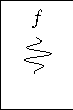
\includegraphics{assets/insets/nolesion_frequency.pdf}};
					\end{axis}
				\end{tikzpicture}
				\caption[Effect of depth and interrogation frequency on magnitude of acoustic body forces]{Effect of depth and interrogation frequency on the magnitude of acoustic body forces developed in tissue. Increasing the interrogation frequency or the focal depth results in lesser body loads experienced by the tissue at the focal point, with the greatest loss of magnitude resulting from focal depth.}
				\label{fig:freq-depth-force}
			\end{figure}

			As Fig. \ref{fig:freq-depth-force} shows, increasing focal depth and probing frequency drastically decreases the magnitude of the force at the focal point of the tissue. In general, forces that are greater in magnitude are ideal as the deflection in the tissue that they cause must be detectable by the same transducer that is applying the forces---if the resulting deflections are too low, the tracking waves sent by the transducer will not be able to distinguish the motion. For the Siemens ACUSON S2000\textsuperscript{\texttrademark}\ machine used in the validation of these studies, this lower limit is quoted as being $\sfrac{1}{100}$ of the applied wavelength, or approximately \SI{1.7}{\um} for a \SI{9}{\MHz} probing frequency \cite{SiemensVirtualTouch}.

			Since the forces developed in the tissue represent a transfer of energy, theoretically increasing the amount of energy input into the system should increase, or at least assist in greater amount of energy being transferred to the tissue. One way of increasing the amount of energy applied to the tissue by the transducer is to increase the size, or the ``aperture'' of the transducer---an aperture of \SI{8}{\cm} will use twice as many physical pulsing elements than an aperture of \SI{4}{\cm}. To study this, the magnitude of the body force at the focal point was studied in simulation as the aperture changed. The results of this study are shown in Fig. \ref{fig:trans-width-force}.

			\begin{figure}[!htb]
				\centering
				\begin{tikzpicture}
					\begin{axis}[
						scale only axis,
						height=2.5in,
						width=\textwidth-\widthof{100}-1in,
						xlabel={ARFI Interrogation Frequency, $f_{ARFI}$ (\si{\MHz})},
						ylabel style={align=center},
						ylabel={Body Force at Focal Point, \\ $F_{b,f}$ (\si{\kN\per\metre\cubed})},
						grid=major,
						legend entries={\textbf{Transducer Width}, $w_{trans} = \SI{4}{\cm}$, $w_{trans} = \SI{8}{\cm}$, $w_{trans} = \SI{10}{\cm}$},
						legend style={legend pos=north east,font=\small,nodes={right}},
						clip=true,
						cycle list name=ColourPlotCycle,
						draw=black, text=black, fill=black]
						\addlegendimage{empty legend};
						\addplot table[y expr=\thisrow{force}*1e-3] {assets/arfi/data/freq_force_width4.dat};
						\addplot table[y expr=\thisrow{force}*1e-3] {assets/arfi/data/freq_force_width8.dat};
						\addplot table[y expr=\thisrow{force}*1e-3] {assets/arfi/data/freq_force_width10.dat};
						\node [anchor=north](c) at (axis cs:3.5,65) {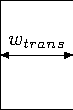
\includegraphics{assets/insets/transducer_width.pdf}};
					\end{axis}
				\end{tikzpicture}
				\caption[Effect of transducer aperture on the magnitude of acoustic radiation force]{Effect of transducer aperture on the magnitude of developed acoustic radiation force at the focal depth of \SI{6}{\cm} for a range of ultrasound interrogation frequencies.}
				\label{fig:trans-width-force}
			\end{figure}

			Surprisingly, there was little consistent effect of the transducer aperture size on the magnitude of the acoustic radiation force that was seen at the focal point. As expected, the greatest and least forces were developed with the lowest and highest frequencies studied, respectively, as per the results found in Fig. \ref{fig:freq-depth-force}. The greatest effect of the transducer aperture size occurred at a frequency of \SI{1}{\MHz} while the least effect of the transducer aperture size occurred at a frequency of \SI{4}{\MHz} which correlate to the greatest and least amount of energy input into the system respectively.

			Another method of increasing the amount of energy transferred into the system is to increase the duration of time that the system is applying pressure to the tissue. In other words, increasing the number of pulse cycles (insonification time) should generate more energy until tissue is under quasi-steady-state insonification. To investigate this, the effect of the number of acoustic pulse cycles---related to the insonification time by equation \ref{equ:insonification_time}---was investigated, with the results shown in Fig. \ref{fig:pulse_cycles_force}.

			\begin{equation}
			\label{equ:insonification_time}
				t_{inson} = \frac{n_c}{f_{applied}}
			\end{equation}

			\begin{figure}[!htb]
				\centering
				\begin{tikzpicture}
					\begin{axis}[
						scale only axis,
						height=2.5in,
						width=\textwidth-\widthof{100}-1in,
						xlabel={Pulse Cycles, $n_c$},
						ylabel style={align=center},
						ylabel={Body Force at Focal Point, \\ $F_{b,f}$ (\si{\kN\per\metre\cubed})},
						grid=major,
						clip=true,
						cycle list name=ColourPlotCycle,
						draw=black, text=black, fill=black]
						\addplot table[y expr=\thisrow{force}*1e-3] {assets/arfi/data/pulse_cycles.dat};
						\node [anchor=south](c) at (axis cs:675,0) {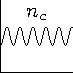
\includegraphics{assets/insets/number_cycles.pdf}};
					\end{axis}
				\end{tikzpicture}
				\caption[Magnitude of developed acoustic radiation force in relation to the number of applied pulse cycles]{Magnitude of the developed acoustic radiation force in relation to the number of applied pulse cycles in tissue at a focal depth of \SI{6}{\cm} using a transducer aperture of \SI{4}{\cm} and source pressure of \SI{3.35}{\MPa}.}
				\label{fig:pulse_cycles_force}
			\end{figure}

			As expected, increasing the number of pulse cycles increased the magnitude of the acoustic radiation force seen at the focal point until the domain reached quasi-steady-state at approximately 300 pulses, or \SI{150}{\us} of insonification. At this point, since the calculation of the acoustic radiation force given in equation \ref{equ:radiation_force} relies on the \emph{average} intensity during the insonification time, increasing the number of pulse cycles has little to no effect on the resulting acoustic radiation force.

			One further way of increasing the energy in the system and thereby increasing the magnitude of the acoustic radiation force at the focal point is to increase the amount of pressure applied by the individual transducer elements.  To investigate this technique, a range of acoustic pulsing element pressures were applied across a range of focal depths and the resulting acoustic radiation force at the focal point was monitored. The results of this study are shown in Fig. \ref{fig:pressure_force}.

			\begin{figure}[!htb]
				\centering
				\begin{tikzpicture}
					\begin{axis}[
						scale only axis,
						height=2.5in,
						width=\textwidth-\widthof{100}-1in,
						xlabel={Focal Depth, $d_f$ (\si{\cm})},
						ylabel style={align=center},
						ylabel={Body Force at Focal Point, \\ $F_{b,f}$ (\si{\kN\per\metre\cubed})},
						grid=major,
						legend entries={\textbf{Source Pressure}, $P_{source} = \SI{4}{\MPa}$, $P_{source} = \SI{5}{\MPa}$, $P_{source} = \SI{6}{\MPa}$, $P_{source} = \SI{7}{\MPa}$, $P_{source} = \SI{8}{\MPa}$},
						legend style={legend pos=north east,font=\small,nodes={right}},
						clip=true,
						cycle list name=ColourPlotCycle,
						draw=black, text=black, fill=black]
						\addlegendimage{empty legend};
						\addplot table[x expr=\thisrow{depth}*100, y expr=\thisrow{force}*1e-3] {assets/arfi/data/focal_force_depth_p4.dat};
						\addplot table[x expr=\thisrow{depth}*100, y expr=\thisrow{force}*1e-3] {assets/arfi/data/focal_force_depth_p5.dat};
						\addplot table[x expr=\thisrow{depth}*100, y expr=\thisrow{force}*1e-3] {assets/arfi/data/focal_force_depth_p6.dat};
						\addplot table[x expr=\thisrow{depth}*100, y expr=\thisrow{force}*1e-3] {assets/arfi/data/focal_force_depth_p7.dat};
						\addplot table[x expr=\thisrow{depth}*100, y expr=\thisrow{force}*1e-3] {assets/arfi/data/focal_force_depth_p8.dat};
						\node [anchor=north](c) at (axis cs:6,240) {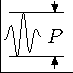
\includegraphics{assets/insets/source_pressure.pdf}};
					\end{axis}
				\end{tikzpicture}
				\caption[Strong dependence on source pressure of focal point force]{Strong dependence on source pressure of focal point force}
				\label{fig:pressure_force}
			\end{figure}

			As Fig. \ref{fig:pressure_force} shows and as was expected, increasing the applied pressure results in greatly increasing the magnitude of the resultant acoustic radiation force developed in the tissue---doubling the applied pressure results in nearly quadrupling the magnitude of the acoustic radiation force at all depths. Note however that a critical measure of the safety of ultrasound is the cavitation pressure of the ultrasonic wave as it travels through the tissue. The safety of cavitation is described by the ``mechanical index'', $MI$, which is calculated according to equation \ref{equ:mechanical_index} \cite{hoskins10} where $P_r$ is the peak rarefaction pressure in the tissue and $f$ is the ultrasound frequency. While an $MI$ less than 0.7 generally means that no cavitation may occur, cavitation is largely only a concern in tissues where cavitation is real possibility---only tissues with embedded gas bodies may cavitate. Since deep tissue injuries are largely focused around the sacrum and heels of tissue, the effects of cavitation in ARFI imaging are not largely relevant.

			\begin{equation}
			\label{equ:mechanical_index}
				MI = \frac{P_r}{\sqrt{f}}
			\end{equation}

			Maximizing the forces developed in the tissue can be detrimental to that tissue's health and well-being. To investigate this, the spatial peak pulse average intensity ($I_{SPPA}$) of the acoustic body load simulations was calculated for the range of depths and frequencies investigated in Fig. \ref{fig:freq-depth-force} and is shown in Fig. \ref{fig:freq-depth-isppa}. Based on a maximum $I_{SPPA}$ exposure of \SI{933}{\W\per\cm\squared} \cite{hoskins10}, the use of ultrasound probes operating at or above \SI{1}{\MHz} and focused at depths greater than \SI{3}{\cm} should be safe for use in examining deep tissue injuries which are generally well separated from the much more sensitive cardiovascular and fetal imaging.

			\begin{figure}[!htb]
				\centering
				\begin{tikzpicture}
					\begin{axis}[
						scale only axis,
						height=2.5in,
						width=\textwidth-\widthof{100}-1in,
						xlabel={Focal Depth, $d_{f}$ (\si{\cm})},
						ylabel style={align=center},
						ylabel={Spatial-Peak Pulse-Average Intensity, \\ $I_{SPPA}$ (\si{\watt\per\cm\squared})},
						grid=major,
						legend entries={\textbf{Interrogation}, \textbf{Frequency}, $f = \SI{1}{\MHz}$, $f = \SI{2}{\MHz}$, $f = \SI{4}{\MHz}$, $f = \SI{6}{\MHz}$, Acceptable limit},
						legend style={legend pos=north east,font=\small,nodes={right}},
						clip=true,
						xmin=0,xmax=10,ymin=0,ymax=2250,
						cycle list name=ColourPlotCycle,
						draw=black, text=black, fill=black]
						\addlegendimage{empty legend};
						\addlegendimage{empty legend};
						\addplot table {assets/arfi/data/depth_isppa_freq1.dat};
						\addplot table {assets/arfi/data/depth_isppa_freq2.dat};
						\addplot table {assets/arfi/data/depth_isppa_freq4.dat};
						\addplot table {assets/arfi/data/depth_isppa_freq6.dat};
						\addplot[mark=none,dashed,ultra thick] plot coordinates {(0, 933) (10, 933)};
						\draw (axis cs:5.5,700) node[right]{Acceptable};
						\draw (axis cs:0.25,1100) node[right]{Unacceptable};
					\end{axis}
				\end{tikzpicture}
				\caption[$I_{SPPA}$ safety measures of ARFI pulses]{The effect of depth and interrogation frequency on the spatial peak pulse average intensity, $I_{SPPA}$. $I_{SPPA}$ is a measure of the safety of high-intensity ultrasound applications, with $I_{SPPA}$ values below \SI{933}{\W\per\cm\squared} considered acceptable for non-cardiovascular and non-fetal imaging.}
				\label{fig:freq-depth-isppa}
			\end{figure}

		\FloatBarrier
		\subsection{Temporal Finite-Element Model of Soft Tissue Deformation}
		\label{subsec:arfi_deformation_results}
			As ARFI imaging relies upon the detection of soft tissue deformation in response to the transducer-applied acoustic radiation force, a key parameter of interest is the magnitude of the deformation generated in the tissue in response to the applied loads. To this end, the temporal finite-element model of soft tissue deformation described in Section \ref{subsec:temporal_fea_arfi} was used to determine the magnitude of the deformation caused by varying acoustic radiation force parameters.

			Fig. \ref{fig:freq-depth-maxDisp} show the relationship between the maximum induced tissue displacement, $\left| v \right|_{max}$, generated by acoustic radiation forces in soft tissue for a range of focal depths and interrogation frequencies. As expected, significantly greater deformation is generated with shallower focal depths. Further, increases in the interrogation frequency generally resulted in lesser displacement induced in the tissue. The results obtained using a \SI{1}{\MHz} interrogation frequency stood apart from the higher frequencies investigated. This is likely due to the excess acoustic radiation force produced at such low frequencies shown in Figs. \ref{fig:freq-depth-force} and \ref{fig:freq-depth-isppa}.

			\begin{figure}[!htb]
				\centering
				\begin{tikzpicture}
					\begin{axis}[
						scale only axis,
						height=2.5in,
						width=\textwidth-\widthof{100}-1in,
						xlabel={Focal Depth, $d_{f}$ (\si{\cm})},
						ylabel style={align=center},
						ylabel={Maximum Induced Tissue \\ Displacement, $\left|v\right|_{max}$ (\si{\micro\metre})},
						grid=major,
						legend entries={\textbf{Interrogation}, \textbf{Frequency}, $f = \SI{1}{\MHz}$, $f = \SI{2}{\MHz}$, $f = \SI{4}{\MHz}$, $f = \SI{6}{\MHz}$},
						legend style={legend pos=north east,font=\small,nodes={right}},
						clip=true,
						cycle list name=ColourPlotCycle,
						draw=black, text=black, fill=black]
						\addlegendimage{empty legend};
						\addlegendimage{empty legend};
						\addplot table[x expr=\thisrow{depth}*100, y expr=\thisrow{maxDisp}*1e6] {assets/arfi/data/depth_maxDisp_freq1.dat};
						\addplot table[x expr=\thisrow{depth}*100, y expr=\thisrow{maxDisp}*1e6] {assets/arfi/data/depth_maxDisp_freq2.dat};
						\addplot table[x expr=\thisrow{depth}*100, y expr=\thisrow{maxDisp}*1e6] {assets/arfi/data/depth_maxDisp_freq4.dat};
						\addplot table[x expr=\thisrow{depth}*100, y expr=\thisrow{maxDisp}*1e6] {assets/arfi/data/depth_maxDisp_freq6.dat};
						\node [anchor=south](c) at (axis cs:1.25,-0.1) {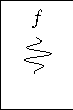
\includegraphics{assets/insets/nolesion_frequency.pdf}};
					\end{axis}
				\end{tikzpicture}
				\caption[ARFI-induced deformation at various depths and interrogation frequencies]{Magnitude of deformation resulting from ARFI interrogation at various focal depths and interrogation frequencies with a transducer aperture of \SI{4}{\cm} and source pressure of \SI{3.35}{\MPa}.}
				\label{fig:freq-depth-maxDisp}
			\end{figure}

			To reiterate the results seen in Fig. \ref{fig:pressure_force}, the maximum induced tissue displacement generated by the applied acoustic radiation force at various focal depths for various source pressures was investigated, the results of which are given in Fig. \ref{fig:pressure_maxDisp}. These results echo the results seen in Fig. \ref{fig:pressure_force}, where doubling the applied pressure resulted in approximately quadrupling the maximum displacement seen in the tissue across all focal depths as was expected.

			\begin{figure}[!htb]
				\centering
				\begin{tikzpicture}
					\begin{axis}[
						scale only axis,
						height=2.5in,
						width=\textwidth-\widthof{100}-1in,
						xlabel={Focal Depth, $d_f$ (\si{\cm})},
						ylabel style={align=center},
						ylabel={Maximum Induced Tissue \\ Displacement, $\left|v\right|_{max}$ (\si{\micro\metre})},
						grid=major,
						legend entries={\textbf{Source Pressure}, $P_{source} = \SI{4}{\MPa}$, $P_{source} = \SI{5}{\MPa}$, $P_{source} = \SI{6}{\MPa}$, $P_{source} = \SI{7}{\MPa}$, $P_{source} = \SI{8}{\MPa}$},
						legend style={legend pos=north east,font=\small},
						clip=true,
						cycle list name=ColourPlotCycle,
						draw=black, text=black, fill=black]
						\addlegendimage{empty legend};
						\addplot table[x expr=\thisrow{depth}*100, y expr=\thisrow{maxDisp}*1e6] {assets/arfi/data/maxDisp_depth_p4.dat};
						\addplot table[x expr=\thisrow{depth}*100, y expr=\thisrow{maxDisp}*1e6] {assets/arfi/data/maxDisp_depth_p5.dat};
						\addplot table[x expr=\thisrow{depth}*100, y expr=\thisrow{maxDisp}*1e6] {assets/arfi/data/maxDisp_depth_p6.dat};
						\addplot table[x expr=\thisrow{depth}*100, y expr=\thisrow{maxDisp}*1e6] {assets/arfi/data/maxDisp_depth_p7.dat};
						\addplot table[x expr=\thisrow{depth}*100, y expr=\thisrow{maxDisp}*1e6] {assets/arfi/data/maxDisp_depth_p8.dat};
						%\addplot[mark=none,dashed,ultra thick] plot coordinates {(3, 1.925) (9, 1.925)};
						\node [anchor=north](c) at (axis cs:6.1,6.15) {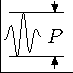
\includegraphics{assets/insets/source_pressure.pdf}};
					\end{axis}
				\end{tikzpicture}
				\caption[ARFI-induced deformation at various depths and source pressures]{Magnitude of deformation resulting from ARFI interrogation at various focal depths and source pressures at an interrogation frequency of \SI{2}{\MHz} with a transducer aperture of \SI{4}{\cm} and source pressure of \SI{3.35}{\MPa}.}
				\label{fig:pressure_maxDisp}
			\end{figure}

			The results given in Fig. \ref{fig:pressure_maxDisp} were further investigated by examining the effect of the interrogation frequency on the maximum induced tissue displacement. As expected, increasing the interrogation frequency resulted in decreases in the magnitude of deformation experienced by the tissue across all source pressures investigated. Further, increasing the amount of source pressure applied by the transducer into the tissue resulted in greater levels of tissue deformation. Of note is that the use of a \SI{1}{\MHz} interrogation frequency affected the magnitude of tissue deformation across the different source pressures much more than any of the higher interrogation frequencies studied, further echoing the results seen in Fig. \ref{fig:freq-depth-maxDisp}.

			\begin{figure}[!htb]
				\centering
				\begin{tikzpicture}
					\begin{axis}[
						scale only axis,
						height=2.5in,
						width=\textwidth-\widthof{100}-1in,
						xlabel={Probing Frequency, $f$ (\si{\MHz})},
						ylabel style={align=center},
						ylabel={Maximum Induced Tissue \\ Displacement, $\left|v\right|_{max}$ (\si{\micro\metre})},
						grid=major,
						legend entries={\textbf{Source Pressure}, $P_{source} = \SI{4}{\MPa}$, $P_{source} = \SI{6}{\MPa}$, $P_{source} = \SI{8}{\MPa}$},
						legend style={legend pos=north east,font=\small},
						clip=true,
						cycle list name=ColourPlotCycle,
						draw=black, text=black, fill=black]
						\addlegendimage{empty legend};
						\addplot table[x expr=\thisrow{frequency}*1e-6, y expr=\thisrow{maxDisp}*1e6] {assets/arfi/data/freq_maxDisp_p4.dat};
						\addplot table[x expr=\thisrow{frequency}*1e-6, y expr=\thisrow{maxDisp}*1e6] {assets/arfi/data/freq_maxDisp_p6.dat};
						\addplot table[x expr=\thisrow{frequency}*1e-6, y expr=\thisrow{maxDisp}*1e6] {assets/arfi/data/freq_maxDisp_p8.dat};
						\node [anchor=north](c) at (axis cs:3.6,7.25) {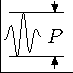
\includegraphics{assets/insets/source_pressure.pdf}};
					\end{axis}
				\end{tikzpicture}
				\caption[ARFI-induced deformation across various interrogation frequencies and source pressures]{Magnitude of deformation resulting from ARFI interrogation at various interrogation frequencies and source pressures at a depth of \SI{6}{\cm} with a transducer aperture of \SI{4}{\cm} and source pressure of \SI{3.35}{\MPa}.}
				\label{fig:freq_pressure_maxDisp}
			\end{figure}

		\FloatBarrier
		\subsection{Numerical Characterization of Acoustic Radiation Force Impulse Imaging}
		\label{subsec:arfi_numerical_characterization}
			Beyond understanding the general nature of acoustic radiation forces in soft tissue, the effects of these forces in the presence of deep tissue injuries must also be characterized for ARFI imaging to become a useful diagnostic tool for such injuries. In order to investigate the suitability of ARFI imaging for the detection of DTI, the procedure outlined in Section \ref{subsec:arfi_method_characterization} was carried out on a range of models with varying parameters of interest. The results of these characterizations are presented here.

			In order to understand the effect of general lesion size on the detection sensitivity of ARFI imaging, hard-boundaried spherical lesions of various radii were placed in a soft tissue domain at a depth of \SI{4}{\cm} and insonated at \SI{2}{\MHz} with an aperture of \SI{4}{\cm} and pressure of \SI{3.35}{\MPa} for \SI{150}{\us} (300 pulse cycles). The results of this characterization are presented in Fig. \ref{fig:arfi_radius}.

			\begin{figure}[!htb]
				\centering
				\characterizationPic{%
					\characterizationPlots{esr}%
						{arfi/data/arfi_radius_r025.dat}%
						{arfi/data/arfi_radius_r050.dat}%
						{arfi/data/arfi_radius_r100.dat}%
						{arfi/data/arfi_radius_r125.dat}%
				}{%
					\characterizationLegend{Lesion Radius}{r_{lesion}}%
						{\SI{2.5}{\mm}}%
						{\SI{5.0}{\mm}}%
						{\SI{10.0}{\mm}}%
						{\SI{12.5}{\mm}}%
				}{spherical_radius}{3.125,0.5}{north west}{ymin=0.5,ymax=2.5}
				\caption[Numerical characterization of ARFI imaging-acquired stiffness ratio with changing lesion radius]{Numerical characterization of the ARFI imaging-acquired stiffness ratios acquired with varying lesion radii for a hard-boundaried lesion at a depth of \SI{4}{\cm} using an ARFI probing frequency of \SI{2}{\MHz}.}
				\label{fig:arfi_radius}
			\end{figure}

			As Fig. \ref{fig:arfi_radius} shows, ARFI imaging was able to detect the presence of both stiff and unstiff lesions of all sizes, however the technique both severely underestimated the stiffness of stiff lesions and overestimated the stiffness of unstiff lesions---leading to the observation that ARFI imaging has a relatively low detection sensitivity with regards to both stiff and unstiff deep tissue injury lesions. Fig. \ref{fig:arfi_radius} also shows that above lesion radii of approximately \SI{2.5}{\mm}, the lesions size does not have any appreciable effect on the detection sensitivity of the technique. Below this limit, however, lesions will be much more difficult to detect as the differences between them and the surrounding tissue are minimized.

			To further corroborate these results, the mean-squared error associated with the various lesion radii was calculated according to equation \ref{equ:mean-squared-error} where $\hat{Y}_i$ are the true lesion stiffness ratios and $Y_i$ are the measured lesion stiffness ratios. The results of this calculation with regards to lesion radius are given in Fig. \ref{fig:arfi_radius_mse}. Figure \ref{fig:arfi_radius_mse} explicitly depicts a greater degree of error for lesions with radii of \SI{2.5}{\mm}, with only marginal improvements in measurement error resulting from increasing the lesion radius beyond \SI{5.0}{\mm}.

			\begin{equation}
				\label{equ:mean-squared-error}
				MSE = \frac{1}{n}\sum_{i=1}^n \left(\hat{Y}_i - Y_i\right)^2
			\end{equation}

			\begin{figure}[!htb]
				\centering
				\begin{tikzpicture}
					\begin{axis}[
						scale only axis,
						height=2.5in,
						width=\textwidth-\widthof{100}-1in,
						major x tick style = transparent,
						ybar=2*\pgflinewidth,
						bar width=28pt,
						ymajorgrids=true,
						xlabel={Lesion Radius, $r$ (\si{\mm})},
						ylabel={Mean Squared Error},
						enlarge x limits=0.25,
						ymin=0,
						symbolic x coords={2.5,5.0,10.0,12.5},
						xtick=data,
						cycle list name=BarColourPlotCycle]
						\addplot table {assets/arfi/data/arfi_radius_mse.dat};
						%\draw[->] (axis cs:2.5, 0.89207) -- (axis cs:12.5, 0.53541);
						\node[anchor=north] at (axis cs:12.5,0.95) {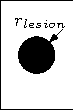
\includegraphics{assets/insets/spherical_radius.pdf}};
					\end{axis}
				\end{tikzpicture}
				\caption[ARFI imaging-acquired lesion stiffness mean squared error related to lesion radius]{Mean squared error between the true and measured lesion stiffness ratios for increasing lesion radii for a hard-boundaried lesion at a depth of \SI{4}{\cm} using an ARFI interrogation frequency of \SI{2}{\MHz}.}
				\label{fig:arfi_radius_mse}
			\end{figure}

			%This may logically be explained by the scales of the acoustic radiation force and the resulting tissue deformations---when healthy tissue deforms by a couple \si{\um} due to applied loading, tissue that is 3 times as stiff will generally deform $\sfrac{1}{3}$ as much, leading to excessively small deformation magnitudes for stiff lesions.

			In order to investigate the effect of lesion depth on detection sensitivity, the use of ARFI imaging to distinguish spherical hard-boundaried lesions with radii of \SI{10}{\mm} was investigated at a range of depths, with the results shown in Fig. \ref{fig:arfi_depth}. As Fig. \ref{fig:arfi_depth} shows, there is almost no dependence of the detection sensitivity on the depth of the lesion. However, it must be noted that the deformations resulting from acoustic radiation force impulses will be of such small magnitudes that they will not be detectable using current ultrasound technology. To understand the limitations of depth in ARFI imaging, please refer to Section \ref{subsec:arfi_deformation_results}.

			\begin{figure}[!htb]
				\centering
				\characterizationPic{%
					\characterizationPlots{esr}%
						{arfi/data/arfi_maxDisp_depth_d2.dat}%
						{arfi/data/arfi_maxDisp_depth_d4.dat}%
						{arfi/data/arfi_maxDisp_depth_d6.dat}%
						{arfi/data/arfi_maxDisp_depth_d8.dat}%
				}{%
					\characterizationLegend{Lesion Depth}{d}%
						{\SI{2}{\cm}}%
						{\SI{4}{\cm}}%
						{\SI{6}{\cm}}%
						{\SI{8}{\cm}}%
				}{spherical_depth}{3.125,0.5}{north west}{ymin=0.5,ymax=2.5}
				\caption[Numerical characterization of ARFI imaging-acquired stiffness ratio with changing lesion depth]{Numerical characterization of the ARFI imaging-acquired stiffness ratios acquired with varying lesion and focal point depths for a hard-boundaried \SI{0.5}{cm} radius lesion using an ARFI probing frequency of \SI{2}{\MHz}.}
				\label{fig:arfi_depth}
			\end{figure}

			Fig. \ref{fig:arfi_depth_mse} portrays the mean-squared-error of the measured lesion stiffness across the various depths examined. Although the variance in error between the different depths is not substantial, both very shallow---lesions at a depth of \SI{2}{\cm} or less---and very deep---lesions at a depth of \SI{8}{\cm} or more---were found to have the greatest measurement error. In shallow tissue, this increase in error may be due to an inability to appropriately focus the acoustic radiation force so close to the transducer whereas in deep tissue, the increase in error is likely due to the reduced magnitude of radiation force present due to the relatively large amount of tissue absorption.

			\begin{figure}[!htb]
				\centering
				\begin{tikzpicture}
					\begin{axis}[
						scale only axis,
						height=2.5in,
						width=\textwidth-\widthof{100}-1in,
						major x tick style = transparent,
						ybar=2*\pgflinewidth,
						bar width=28pt,
						ymajorgrids=true,
						xlabel={Lesion Depth, $d$ (\si{\cm})},
						ylabel={Mean Squared Error},
						enlarge x limits=0.25,
						ymin=0, ymax=0.9,
						xtick=data,
						cycle list name=BarColourPlotCycle]
						\addplot table[x expr=\thisrow{depth}*100] {assets/arfi/data/arfi_depth_mse.dat};
						\node[anchor=south] at (axis cs:8,0.6) {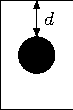
\includegraphics{assets/insets/spherical_depth.pdf}};
					\end{axis}
				\end{tikzpicture}
				\caption[ARFI imaging-acquired lesion stiffness mean squared error related to lesion depth]{Mean squared error between the true and measured lesion stiffness ratios for increasing lesion depths for a hard-boundaried \SI{0.5}{cm} radius lesion using an ARFI interrogation frequency of \SI{2}{\MHz}.}
				\label{fig:arfi_depth_mse}
			\end{figure}

			Since the aforementioned hard-boundaried, spherical lesion cases represent simplifications of reality designed to obtain a general understanding of the ARFI technique, models representing more complicated geometry were also studied. Fig. \ref{fig:arfi_blur} shows the simulated lesion stiffness ratios for a set of lesions with radii of \SI{10}{\mm} at a depth of \SI{4}{\cm} with blurred boundaries as described in Section \ref{subsec:arfi_method_characterization}. As Fig. \ref{fig:arfi_blur} shows, there is no reliance of the detection sensitivity on the blur radius of the lesion, with the results shown repeating the results seen in Figs. \ref{fig:arfi_radius} and \ref{fig:arfi_depth}.

			\begin{figure}[!htb]
				\centering
				\characterizationPic{%
					\characterizationPlots{esr}%
						{arfi/data/arfi_blur_radius_r25.dat}%
						{arfi/data/arfi_blur_radius_r50.dat}%
						{arfi/data/arfi_blur_radius_r75.dat}%
				}{%
					\characterizationLegend{Blur Radius}{b_r}%
						{\SI{2.5}{\mm}}%
						{\SI{5.0}{\mm}}%
						{\SI{7.5}{\mm}}%
				}{blur_radius}{3.125,0.5}{north west}{ymin=0.5,ymax=2.5}
				\caption[Numerical characterization of ARFI imaging-acquired stiffness ratio with blurred lesions]{Numerical characterization of the ARFI imaging-acquired stiffness ratios acquired with varying lesion and focal point depths for a blurred \SI{1.0}{cm} radius lesion at a depth of \SI{4}{\cm} using an ARFI interrogation frequency of \SI{2}{\MHz}.}
				\label{fig:arfi_blur}
			\end{figure}

			The mean-squared error shown in Fig. \ref{fig:arfi_blur_mse} further supports this conclusion, with the error between different blur radii differing by just over \SI{1}{\percent}. This lack of sensitivity on the degree of lesion blurring presents a significant advantage over quasi-static elastography as it allows even lesions without well-defined boundaries to be detected.

			\begin{figure}[!htb]
				\centering
				\begin{tikzpicture}
					\begin{axis}[
						scale only axis,
						height=2.5in,
						width=\textwidth-\widthof{100}-1in,
						major x tick style = transparent,
						ybar=2*\pgflinewidth,
						bar width=28pt,
						ymajorgrids=true,
						xlabel={Lesion Blur Radius, $b_r$ (\si{\mm})},
						ylabel={Mean Squared Error},
						enlarge x limits=0.25,
						ymin=0, xmax=8.5,
						xtick=data,
						cycle list name=BarColourPlotCycle]
						\addplot table[x expr=\thisrow{blur}*1000] {assets/arfi/data/arfi_blur_mse.dat};
						\node[anchor=north] at (axis cs:9,0.6) {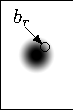
\includegraphics{assets/insets/blur_radius.pdf}};
					\end{axis}
				\end{tikzpicture}
				\caption[ARFI imaging-acquired lesion stiffness mean squared error related to lesion blurring]{Mean squared error between the true and measured lesion stiffness ratios for increasing lesion depths for a blurred \SI{1.0}{cm} radius lesion at a depth of \SI{4}{\cm} using an ARFI interrogation frequency of \SI{2}{\MHz}.}
				\label{fig:arfi_blur_mse}
			\end{figure}

			It may also be possible that a diseased region of tissue is not a singular, continuous lesionous region, but rather an amalgamation of numerous small lesions or damaged tissue which collectively compose a larger lesionous region. To investigate the effect such a phenomenon would have on the detection sensitivity of ARFI imaging, the density and size of numerous small, clustered lesions were varied in models and the resulting measured stiffness ratios were investigated. Fig. \ref{fig:arfi_cluster_density} shows the characterization of the lesion cluster density---how many lesions are present per unit area---for densities ranging from \SI{10}{\per\cm\squared} to \SI{40}{\per\cm\squared} with small lesions of radius \SI{1.0}{\mm}. The centre of the lesionous regions were located at a depth of \SI{4}{\cm} in an overall region with a radius of \SI{10}{\mm}.

			\begin{figure}[!htb]
				\centering
				\characterizationPic{%
					\characterizationPlots{esr}%
						{arfi/data/arfi_cluster_dens_d10.dat}%
						{arfi/data/arfi_cluster_dens_d20.dat}%
						{arfi/data/arfi_cluster_dens_d30.dat}%
						{arfi/data/arfi_cluster_dens_d40.dat}%
				}{%
					\characterizationLegend{Cluster Density}{b_\rho}%
						{\SI{10}{\per\cm\squared}}%
						{\SI{20}{\per\cm\squared}}%
						{\SI{30}{\per\cm\squared}}%
						{\SI{40}{\per\cm\squared}}%
				}{cluster_density}{3.125,0.5}{north west}{ymin=0.5,ymax=2.5}
				\caption[Numerical characterization of ARFI imaging-acquired stiffness ratio with clustered lesions]{Numerical characterization of the ARFI imaging-acquired stiffness ratios acquired with varying cluster densities for clustered \SI{1}{\mm} radius lesions within a \SI{1.0}{cm} radius at a depth of \SI{4}{\cm} using an ARFI interrogation frequency of \SI{2}{\MHz}.}
				\label{fig:arfi_cluster_density}
			\end{figure}

			As Fig. \ref{fig:arfi_cluster_density} shows, increasing the cluster density results in monotonically increasing the detection sensitivity of the ARFI technique. This is as expected, as increasing the cluster density increases the total area contributing to the modified tissue stiffness in the region, which in turn allows the ARFI technique to more readily distinguish the lesion. These results are further shown by the mean-squared error shown in Fig. \ref{fig:arfi_cluster_density_mse} which shows the decrease in error attributed to increases in lesion cluster densities.

			\begin{figure}[!htb]
				\centering
				\begin{tikzpicture}
					\begin{axis}[
						scale only axis,
						height=2.5in,
						width=\textwidth-\widthof{100}-1in,
						major x tick style = transparent,
						ybar=2*\pgflinewidth,
						bar width=28pt,
						ymajorgrids=true,
						xlabel={Lesion Cluster Density, $b_\rho$ (\si{\per\cm\squared})},
						ylabel={Mean Squared Error},
						enlarge x limits=0.25,
						ymin=0,
						xtick=data,
						cycle list name=BarColourPlotCycle]
						\addplot table {assets/arfi/data/arfi_cluster_dens_mse.dat};
						\node[anchor=north] at (axis cs:40,0.95) {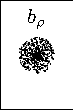
\includegraphics{assets/insets/cluster_density.pdf}};
					\end{axis}
				\end{tikzpicture}
				\caption[ARFI imaging-acquired lesion stiffness mean squared error related to small lesion cluster density]{Mean squared error between the true and measured lesion stiffness ratios for increasing lesion cluster density for clustered \SI{1}{\mm} radius lesions within a \SI{1.0}{cm} radius at a depth of \SI{4}{\cm} using an ARFI interrogation frequency of \SI{2}{\MHz}.}
				\label{fig:arfi_cluster_density_mse}
			\end{figure}

			Another method to alter the ratio of damaged to healthy tissue within the lesionous region is to alter the size of the individual lesions that comprise that region. This characterization was carried out using small lesions with radii ranging from \SI{0.5}{\mm} to \SI{1.5}{\mm} at a cluster density of \SI{30}{\per\cm\squared}, with the results given in Fig. \ref{fig:arfi_cluster_radius}.

			\begin{figure}[!htb]
				\centering
				\characterizationPic{%
					\characterizationPlots{esr}%
						{arfi/data/arfi_cluster_radius_r05.dat}%
						{arfi/data/arfi_cluster_radius_r10.dat}%
						{arfi/data/arfi_cluster_radius_r15.dat}%
				}{%
					\characterizationLegend{Clustered Lesion Radii}{r_{bl}}%
						{\SI{0.5}{\mm}}%
						{\SI{1.0}{\mm}}%
						{\SI{1.5}{\mm}}%
				}{cluster_radius}{3.125,0.5}{north west}{ymin=0.5,ymax=2.5}
				\caption[Numerical characterization of ARFI imaging-acquired stiffness ratio with clustered lesions]{Numerical characterization of the ARFI imaging-acquired stiffness ratios acquired with varying clustered lesion radii for clustered lesions with a density of \SI{30}{\per\cm\squared} within a \SI{1.0}{cm} radius at a depth of \SI{4}{\cm} using an ARFI interrogation frequency of \SI{2}{\MHz}.}
				\label{fig:arfi_cluster_radius}
			\end{figure}

			As Fig, \ref{fig:arfi_cluster_radius} shows, decreasing the individual lesion radii in the clustered model substantially decreased the detection sensitivity of the ARFI technique, again echoing the previous results where decreasing the ratio of damaged to healthy tissue in the lesionous region results in lesser detection sensitivity. This is confirmed by examining the mean-squared error of the results, which shows monotonically decreasing errors for monotonically increasing individual lesion radii.

			\begin{figure}[!htb]
				\centering
				\begin{tikzpicture}
					\begin{axis}[
						scale only axis,
						height=2.5in,
						width=\textwidth-\widthof{100}-1in,
						major x tick style = transparent,
						ybar=2*\pgflinewidth,
						bar width=28pt,
						ymajorgrids=true,
						xlabel={Clustered Lesion Radius, $r_{bl}$ (\si{\mm})},
						ylabel={Mean Squared Error},
						enlarge x limits=0.25,
						ymin=0,
						xtick=data,
						cycle list name=BarColourPlotCycle]
						\addplot table[x expr=\thisrow{radius}*1000] {assets/arfi/data/arfi_cluster_radius_mse.dat};
						\node[anchor=north] at (axis cs:1.5,1.1) {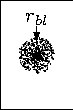
\includegraphics{assets/insets/cluster_radius.pdf}};
					\end{axis}
				\end{tikzpicture}
				\caption[ARFI imaging-acquired lesion stiffness mean squared error related to small lesion cluster density]{Mean squared error between the true and measured lesion stiffness ratios for increasing clustered lesion radii for clustered lesions with a density of \SI{30}{\per\cm\squared} within a \SI{1.0}{cm} radius at a depth of \SI{4}{\cm} using an ARFI interrogation frequency of \SI{2}{\MHz}.}
				\label{fig:arfi_cluster_radius_mse}
			\end{figure}

			While the aforementioned studies investigated generally spherical lesionous regions, this is unlikely to be the case in a real soft tissue domain. To further investigate ARFI imaging, a model utilizing complicated geometry arising from the combination of the MRI-acquired geometry of a deep tissue injury with the anatomical distribution of fat, muscle, and bone obtained from the Visible Human project \cite{visiblehuman} was created as described in Section \ref{subsec:arfi_method_characterization}. To investigate the effect of lesion size in this model, the lesion size, $\diameter L$, was varied between \SI{2.5}{\mm} and \SI{12.5} with the lesion being placed at a depth of \SI{6}{\cm}. The results of this characterization are shown in Fig. \ref{fig:arfi_human_radius}.

			\begin{figure}[!htb]
				\centering
				\characterizationPic{%
					\characterizationPlots{esr}%
						{arfi/data/arfi_human_radius_r025.dat}%
						{arfi/data/arfi_human_radius_r050.dat}%
						{arfi/data/arfi_human_radius_r100.dat}%
						{arfi/data/arfi_human_radius_r125.dat}%
				}{%
					\characterizationLegend{Lesion Width}{\diameter L}%
						{\SI{5}{\mm}}%
						{\SI{10}{\mm}}%
						{\SI{20}{\mm}}%
						{\SI{25}{\mm}}%
				}{human_width}{0.35,1.2}{south east}
				\caption[Numerical characterization of ARFI imaging-acquired stiffness ratio with changing lesion radii in a visible human model]{Numerical characterization of ARFI imaging-acquired stiffness ratio with changing lesion radii for MRI-acquired lesion geometry in a Visible Human model at a depth of \SI{6}{\cm} using an ARFI interrogation frequency of \SI{2}{\MHz}.}
				\label{fig:arfi_human_radius}
			\end{figure}

			As Fig. \ref{fig:arfi_human_radius} shows, decreasing the lesion width in the Visible Human model resulted in a decreased detection sensitivity which was echoed by the mean-square error of the results shown in Fig. \ref{fig:arfi_human_radius_mse}. The detection sensitivity decreases with half-widths less than \SI{10}{\mm} in the Visible Human model as opposed to radii of \SI{5}{\mm} as found with the spherical lesion embedded in general soft tissue seen in Fig. \ref{fig:arfi_radius}. Although the reason for this is not immediately clear, possible differences lay in the depth at which the lesions were imaged at: the Visible Human model placed the lesion at a depth of \SI{6}{\cm} so as to have it lay immediately superior to the ischial tuberosity while the results for the spherical lesion were taken at a depth of \SI{4}{\cm}. Further, comparing the half-width of the Visible Human lesion to the radius of the spherical lesion may introduce errors as the overall area of lesionous tissue were different.

			\begin{figure}[!htb]
				\centering
				\begin{tikzpicture}
					\begin{axis}[
						scale only axis,
						height=2.5in,
						width=\textwidth-\widthof{100}-1in,
						major x tick style = transparent,
						ybar=2*\pgflinewidth,
						bar width=28pt,
						ymajorgrids=true,
						xlabel={Lesion Width, $\diameter L$ (\si{\mm})},
						ylabel={Mean Squared Error},
						enlarge x limits=0.25,
						ymin=0, ymax=1.4,
						symbolic x coords={5.0,10.0,20.0,25.0},
						xtick=data,
						cycle list name=BarColourPlotCycle]
						\addplot table {assets/arfi/data/arfi_human_radius_mse.dat};
						\node[anchor=north] at (axis cs:25.0,1.4) {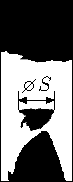
\includegraphics{assets/insets/human_width.pdf}};
					\end{axis}
				\end{tikzpicture}
				\caption[ARFI imaging-acquired lesion stiffness mean squared error related to MRI-acquired lesion size in a Visible Human model]{Mean squared error between the true and measured lesion stiffness ratios for increasing lesion radii for MRI-acquired lesion geometry in a Visible Human model at a depth of \SI{6}{\cm} using an ARFI interrogation frequency of \SI{2}{\MHz}.}
				\label{fig:arfi_human_radius_mse}
			\end{figure}

			Numerical values for the characterization plots presented here are given in Section \ref{appsec:dt_arfi} of Appendix \ref{app:data_tables}.

		\FloatBarrier
		\subsection{Physical Phantom Validation}
		\label{subsec:arfi_validation_results}
			In order to determine if the results presented in Section \ref{subsec:arfi_numerical_characterization} represent valid simulations, validation experiments were carried out on a physical tissue mimicking phantom as described in Section \ref{subsec:arfi_physical_phantom}. Fig. \ref{fig:arfi_phantom_validation_nominal} shows the result of these experiments.

			\begin{figure}[!htb]
				\centering
				\begin{tikzpicture}
					\begin{axis}[
						scale only axis,
						height=2.5in,
						width=\textwidth-\widthof{100}-1in,
						xlabel={Nominal Stiffness Ratio, $E_{rel,nom}$},
						ylabel style={align=center},
						ylabel={Experimentally Measured \\ Stiffness Ratio, $E_{exp,measured}$},
						legend entries={Results, Ideal},
						legend style={legend pos=south east,font=\small},grid=major,clip=true,cycle list name=ColourPlotCycle,
						xmin=0, xmax=4,
						ymin=0, ymax=4,
						draw=black, text=black, fill=black]
							\addplot+[
								error bars/.cd,
								y dir=both,
								y explicit,
								error bar style={ultra thick},
								error mark options={
									rotate=90,
									mark size=8pt,
									ultra thick
								}] table[y error plus=upper, y error minus=lower] {assets/arfi/data/arfi_experiment_nominal.dat};
							\addplot[mark=none,dashed,ultra thick] plot coordinates {(0, 0) (4, 4)};
							\node (c) at (axis cs:0.5,3) {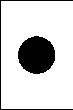
\includegraphics{assets/insets/spherical.pdf}};
					\end{axis}
				\end{tikzpicture}
				\caption[Experimental ARFI model results]{Relation between nominally reported strain ratios of the tissue mimicking phantom and experimentally measured strain ratios for a lesion at a depth of \SI{3.5}{\cm} and diameter of \SI{2.0}{\cm}. Error bars represent the range of measurements acquired.}
				\label{fig:arfi_phantom_validation_nominal}
			\end{figure}

			As the results seen in Fig. \ref{fig:arfi_phantom_validation_nominal} show, ARFI imaging was found experimentally to significantly underestimate the stiffness of the stiffest lesions investigated---lesions with nominal stiffnesses of 3.2. For all other lesions investigated, ARFI imaging was shown to overestimate the lesion stiffness slightly. Although it is possible that the true stiffness ratio of the lesions in the phantom do not perfectly align with the manufacturer-reported nominal values, it is also possible that the acoustic radiation force developed by the ARFI transducer was not enough to substantially deform the stiffest of lesions, leading to the stiffness being underestimated.

			Fig. \ref{fig:arfi_phantom_validation} compares the experimentally-acquired lesion stiffness ratios against measured stiffness ratios arising from parametrically identical simulated lesions. As Fig. \ref{fig:arfi_phantom_validation} shows, although the experimentally measured stiffness ratios align well with the simulated stiffness ratios for relatively unstiff lesions ($E_{rel} < 1$), the simulated ARFI procedure was found to underestimate the stiffness of the stiff lesions that were investigated ($E_{rel} > 1$). The exact cause of this disparity is unclear and future work must be done in order to remedy this in the simulations that were performed in order to accurately understand ARFI imaging.

			\begin{figure}[!htb]
				\centering
				\begin{tikzpicture}
					\begin{axis}[
						scale only axis,
						height=2.5in,
						width=\textwidth-\widthof{100}-1in,
						xlabel={Experimentally Measured Stiffness Ratio, $E_{exp,measured}$},
						ylabel style={align=center},
						ylabel={Simulated Measured \\ Stiffness Ratio, $E_{sim,measured}$},
						legend entries={Results, Ideal},
						legend style={legend pos=south east,font=\small},grid=major,clip=true,cycle list name=ColourPlotCycle,
						xmin=0, xmax=4,
						ymin=0, ymax=4,
						draw=black, text=black, fill=black]
							\addplot+[
								error bars/.cd,
								x dir=both,
								x explicit,
								error bar style={ultra thick},
								error mark options={
									rotate=90,
									mark size=8pt,
									ultra thick
								}] table[x error plus=upper, x error minus=lower] {assets/arfi/data/arfi_experiment.dat};
							\addplot[mark=none,dashed,ultra thick] plot coordinates {(0, 0) (4, 4)};
							\node (c) at (axis cs:0.5,3) {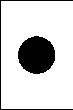
\includegraphics{assets/insets/spherical.pdf}};
					\end{axis}
				\end{tikzpicture}
				\caption[Experimental validation of ARFI imaging model results]{Relation between simulated measured strain ratios and experimental measured strain ratios for a lesion at a depth of \SI{3.5}{\cm} and diameter of \SI{2.0}{\cm}.}
				\label{fig:arfi_phantom_validation}
			\end{figure}

	\section{Conclusion}
		The results presented in Section \ref{sec:arfi_results} represent a numerical characterization of the use of acoustic radiation force impulse imaging for the detection of deep tissue injuries including: the distribution of acoustic radiation force generated by transducers; the generalized tissue response to these acoustic radiation forces; and the use of ARFI imaging to distinguish both early and formative deep tissue injuries from surrounding healthy tissue. Although the principles of operation for ARFI imaging and quasi-static ultrasound elastography are the same---detecting the relative magnitude of deformation in regions of tissue in response to externally applied forces---ARFI imaging presents a key advantage over quasi-static ultrasound elastography in that it allows much greater inter-operator reliability and repeatability. ARFI imaging generates deformation within tissue automatically and without dependence on the operator which is key to developing a successful diagnostic modality.

		A key parameter relating to the ability of acoustic radiation force impulses to generate adequate body loads in tissue is the depth at which the radiation force is focused at---increasing depth was found to induce the greatest reduction in the magnitude of the radiation forces and the subsequent magnitude of tissue deformation. This is of concern, as once the magnitude of tissue deformation becomes small enough these deformations will no longer be able to be tracked using conventional ultrasound beams. In order to counteract this, lower frequencies and greater transmit pressures may be used, however care must be taken to ensure the safety of patients undergoing such techniques as the energy resulting from acoustic radiation has the potential to result in tissue damage.

		The results shown in Section \ref{subsec:arfi_numerical_characterization} show that ARFI imaging is a suitable technique for differentiating both stiff and unstiff lesions from surrounding healthy tissue which may be indicative of deep tissue injury formation and progression. Overall, the detection sensitivity of ARFI imaging is less than ideal with the stiffness of stiff lesions consistently underestimated and the stiffness of unstiff lesions consistently overestimated. ARFI imaging was found to not be dependent on lesion radius above radii of approximately \SI{2.5}{\mm} and aside from issues with deformation magnitude, the depth of the lesions has no appreciable effect on their detection ability. The amount of lesion blur also did not affect the detection sensitivity, which is advantageous for detecting lesions without clearly defined boundaries. Regions of clustered deep tissue injury lesions were detectable however decreasing the ratio of diseased to healthy tissue area in the lesion resulted in lower detection sensitivities. Lesions were still detectable in the complicated model of MRI-acquired geometry embedded within soft tissue layout extracted from the Visible Human project, although to a slightly lesser extent than uncomplicated hard-boundaried spherical lesions. The overall technique was experimentally validated, however it was found that the simulated lesions underestimated the lesion stiffness compared to their parametrically-identical experimental counterparts.

		Future work involving ARFI imaging should investigate the disparity between the experimentally-acquired lesion stiffness ratios and the simulated lesion stiffness ratios in order to increase the validity of the models. In order to truly advance the technology toward its clinical adoption, experimental studies in animals and humans with known deep tissue injuries must be carried out to determine the applicability of ARFI imaging in a real-world setting.

\bibcomplete{references}